%\documentclass[sigconf,anonymous, review]{acmart}
\documentclass[sigconf]{acmart} %review %anonymous

\usepackage{subcaption}
%\usepackage[caption=true,font=small]{subfig}
\usepackage{booktabs} % For formal tables
\usepackage[linesnumbered,vlined,ruled]{algorithm2e}
\usepackage{amsmath,amssymb,amsfonts}
\DeclareMathOperator*{\argmax}{arg\,max}
\DeclareMathOperator*{\mean}{mean}
% Copyright
%\setcopyright{none}
%\setcopyright{acmcopyright}
%\setcopyright{acmlicensed}
\setcopyright{rightsretained}
%\setcopyright{usgov}
%\setcopyright{usgovmixed}
%\setcopyright{cagov}
%\setcopyright{cagovmixed}
\usepackage{mathtools}
\usepackage{multirow}
\usepackage{tikz}

\DeclarePairedDelimiter\ceil{\lceil}{\rceil}
\DeclarePairedDelimiter\floor{\lfloor}{\rfloor}
%\DeclarePairedDelimiter\parentheses{\(}{\)}

\newif\ifstartedinmathmode
\newcommand\encircled[1]{%
  \relax\ifmmode\startedinmathmodetrue\else\startedinmathmodefalse\fi%
  \tikz[baseline,anchor=base]{%
  \node[draw,circle,outer sep=0pt,inner sep=.2ex]
    {\ifstartedinmathmode$#1$\else#1\fi};}%
}

% DOI
%\acmDOI{10.475/123_4}

% ISBN
%\acmISBN{123-4567-24-567/08/06}

%Conference
\acmConference[]{CDNG 2020}{March 2020}{Brisbane, Australia}
\acmYear{2020}
\copyrightyear{2020}

%\acmArticle{4}
%\acmPrice{15.00}

% These commands are optional
%\acmBooktitle{Transactions of the ACM Woodstock conference}
%\editor{Jennifer B. Sartor}
%\editor{Theo D'Hondt}
%\editor{Wolfgang De Meuter}

\begin{document}
	
%\balance

\title{Spatial Privacy Leakage in 3D Mixed Reality Data}
%\titlenote{Produces the permission block, and
%  copyright information}
%\subtitle{Extended Abstract}
%\subtitlenote{The full version of the author's guide is available as
 % \texttt{acmart.pdf} document}

\author{Jaybie Agullo de Guzman}
\orcid{0000-0002-2816-7721}
\affiliation{%
  \institution{Data 61, CSIRO \&\\
  University of New South Wales}
  \city{Sydney}
\country{Australia}
}
\email{jaybie.deguzman@data61.csiro.au}

\author{Kanchana Thilakarathna}
\affiliation{%
  \institution{University of Sydney \&\\ Data 61, CSIRO}
  %\streetaddress{P.O. Box 1212}
  %\city{Dublin}
  \city{Sydney}
	\country{Australia}
  %\postcode{43017-6221}
}
\email{kanchana.thilakarathna@sydney.edu.au}

\author{Aruna Seneviratne}
\affiliation{%
  \institution{University of New South Wales \&\\ Data 61, CSIRO}
%  \streetaddress{1 Th{\o}rv{\"a}ld Circle}
  \city{Sydney}
  \country{Australia}
}
\email{a.seneviratne@unsw.edu.au}

% The default list of authors is too long for headers.
\renewcommand{\shortauthors}{J. de Guzman, K. Thilakarathna, \& A. Seneviratne}

\begin{abstract}
We have seen a rise in augmented and mixed reality (AR or MR) applications, devices, and platforms in recent years. These technologies require spatial understanding to detect physical objects or surfaces often including their structural (i.e. spatial geometry) and photometric (e.g. color, and texture) attributes extracted from captured 3D spatial data. Then, these AR/MR applications can render virtual or synthetic objects that seemingly inhabit the real world, and, in some cases, even allowing interactions between physical and virtual objects. However, this capability poses unprecedented risks to user privacy, and we are only starting to realize these risks. Aside from objects being detected, captured 3D spatial data may also reveal other sensitive information the user did not intend to be captured such as the location they are in or the sensitive objects around them. Current privacy protection measures are primarily aimed towards known and well-utilised data types (i.e. location, on-line activity, biometric, and so on) while a few works have focused on looking into the security and privacy risks of and providing protection on MR data, particularly on 3D MR data. Thus, recently, we have been working on (1) revealing and quantifying the spatial privacy leakage from 3D MR data capture, and (2) using the derived metrics to inform the design of privacy preserving measures to be applied over captured 3D MR spatial data. In our latest work, we investigate \textit{conservative releasing} of generalized planes as a form of spatial privacy protection. %We have revealed how easy it is to 
\end{abstract}

%
% The code below should be generated by the tool at
% http://dl.acm.org/ccs.cfm
% Please copy and paste the code instead of the example below.
%
 \begin{CCSXML}
	<ccs2012>
	<concept>
	<concept_id>10003120.10003121.10003124.10010392</concept_id>
	<concept_desc>Human-centered computing~Mixed / augmented reality</concept_desc>
	<concept_significance>500</concept_significance>
	</concept>
	<concept>
	<concept_id>10002978.10003018.10003021</concept_id>
	<concept_desc>Security and privacy~Information accountability and usage control</concept_desc>
	<concept_significance>300</concept_significance>
	</concept>
	<concept>
	<concept_id>10002978.10003029.10011150</concept_id>
	<concept_desc>Security and privacy~Privacy protections</concept_desc>
	<concept_significance>300</concept_significance>
	</concept>
	<concept>
	<concept_id>10010147.10010178.10010224.10010226.10010239</concept_id>
	<concept_desc>Computing methodologies~3D imaging</concept_desc>
	<concept_significance>300</concept_significance>
	</concept>
	</ccs2012>
\end{CCSXML}

\ccsdesc[500]{Human-centered computing~Mixed / augmented reality}
\ccsdesc[300]{Security and privacy~Information accountability and usage control}
\ccsdesc[300]{Security and privacy~Privacy protections}
\ccsdesc[300]{Computing methodologies~3D imaging}


\keywords{}


\maketitle

%\RestyleAlgo{boxruled}
\section{BACKGROUND \& MOTIVATION}

%Most mobile MR development platforms (i.e. ARCore, and ARKit) utilise a form of \textit{visual odometry} %\cite{yousif2015overview}
%combined with motion or inertial information to map the device's position relative to the real-world, while dedicated HMDs (i.e. HoloLens), leverage multiple cameras with depth sensors to understand the environment and create a virtual 3D map. Once a good mapping has been created, the virtual space (or a coordinate system) is shared with applications to allow synthetic or augmented content to interact with the physical world such as \textit{anchoring} a virtual object on your desk.% This mapping is usually in the form of a 3D \textit{point cloud}.% accompanied by normal vectors to signify orientation of the points which allows for easier surface detection.

% The opening discussion focuses on the necessary processes that delivers the MR services.
AR/MR platforms such as Google ARCore, %\cite{arcore}, 
Apple ARKit, % \cite{arkit}, 
and Windows Mixed Reality API %\cite{windowsMRdev} 
requires spatial understanding of the user environment in order to deliver virtual augmentations that seemingly inhabit the real world, and, in some immersive examples, even interact with physical objects.\footnote{ARKit, \url{https://developer.apple.com/documentation/arkit};
ARCore, \url{https://developers.google.com/ar/};
Windows MR, \url{https://www.microsoft.com/en-au/windows/windows-mixed-reality}. For the rest of the paper, we will be collectively referring to AR and MR as MR.} Fig. \ref{fig:generic-pipeline} presents a generic MR process or information flow diagram. The device captures the spatial information of the space and stores it as a 3D spatial map or point cloud (labelled $S_i$ in Fig. \ref{fig:generic-pipeline}). The point cloud can be accompanied by mesh information to indicate how the points, when connected, represent surfaces and other structures in the user environment. Afterwards, the point cloud is provided to applications to provide spatial understanding and deliver their intended functions, say, augmenting a virtual monster on the floor. However, these 3D point clouds may contain sensitive information which the user did not intend to expose which can, then, be accessed by a potential adversary (labelled $J$ in Fig.\ref{fig:generic-pipeline}), and be further utilized for functionalities beyond the application's intended function such as aggressive localized advertisements. And, so far, there are no mechanisms in place that ensure user data privacy in MR platforms.%Captured visual information are mapped to a digital 3D spatial map with the aid of additional motion and/or depth sensor information. This 3D spatial map is usually stored as a set of 3D points, i.e. $(x, y, z)$, which may be accompanied by additional attributes such as orientation (i.e. normal vectors) or photometric information (e.g. RGB, SIFT feature vector, etc.).  further accompanied by a mesh information that tells which points, when connected, form surfaces.
%However, even with only the 3D point information left -- even without additional attributes -- much of the objects within the space or the space itself can still be identified.

\begin{figure}[t]
	\centering
	\vspace{2mm}
	\begin{subfigure}{\columnwidth}
		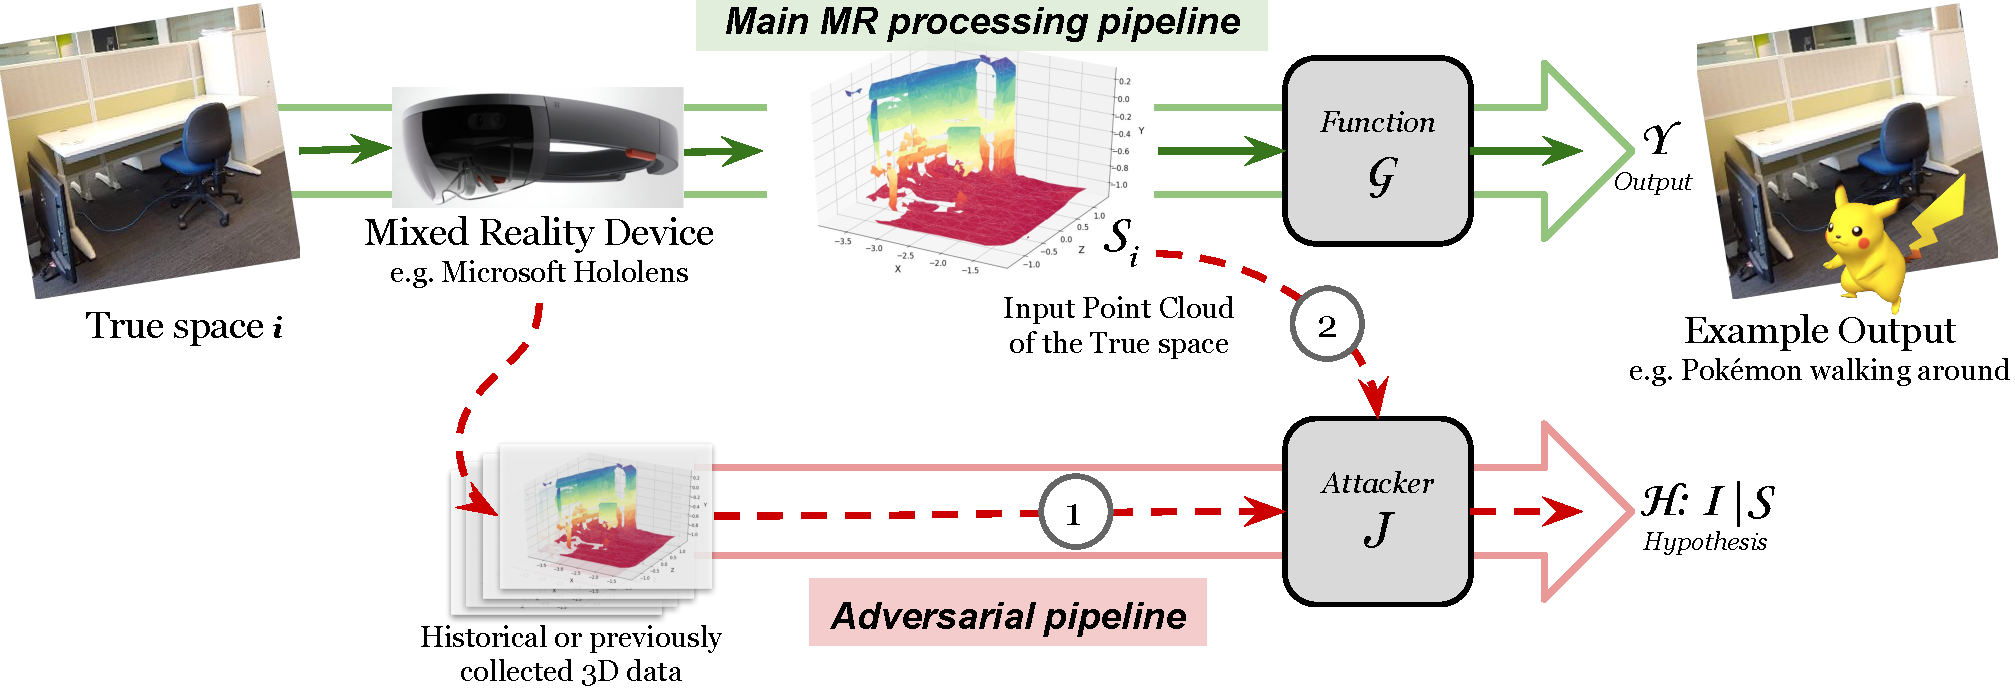
\includegraphics[width=\columnwidth]{figures/adversary-model-pipeline-v6-revised-a.pdf}
		\caption{\small Information flow diagram (following the green solid arrows) for an intended MR function $G$, with an attacker $J$ which can perform adversarial spatial inference: (1) adversarial inference \textit{modeling} or \textit{learning} from, say, historical 3D data, and (2) adversarial inference or \textit{matching} over currently released 3D data}
		\label{fig:generic-pipeline}
    	\vspace{3mm}
	\end{subfigure}
	\begin{subfigure}{\columnwidth}
		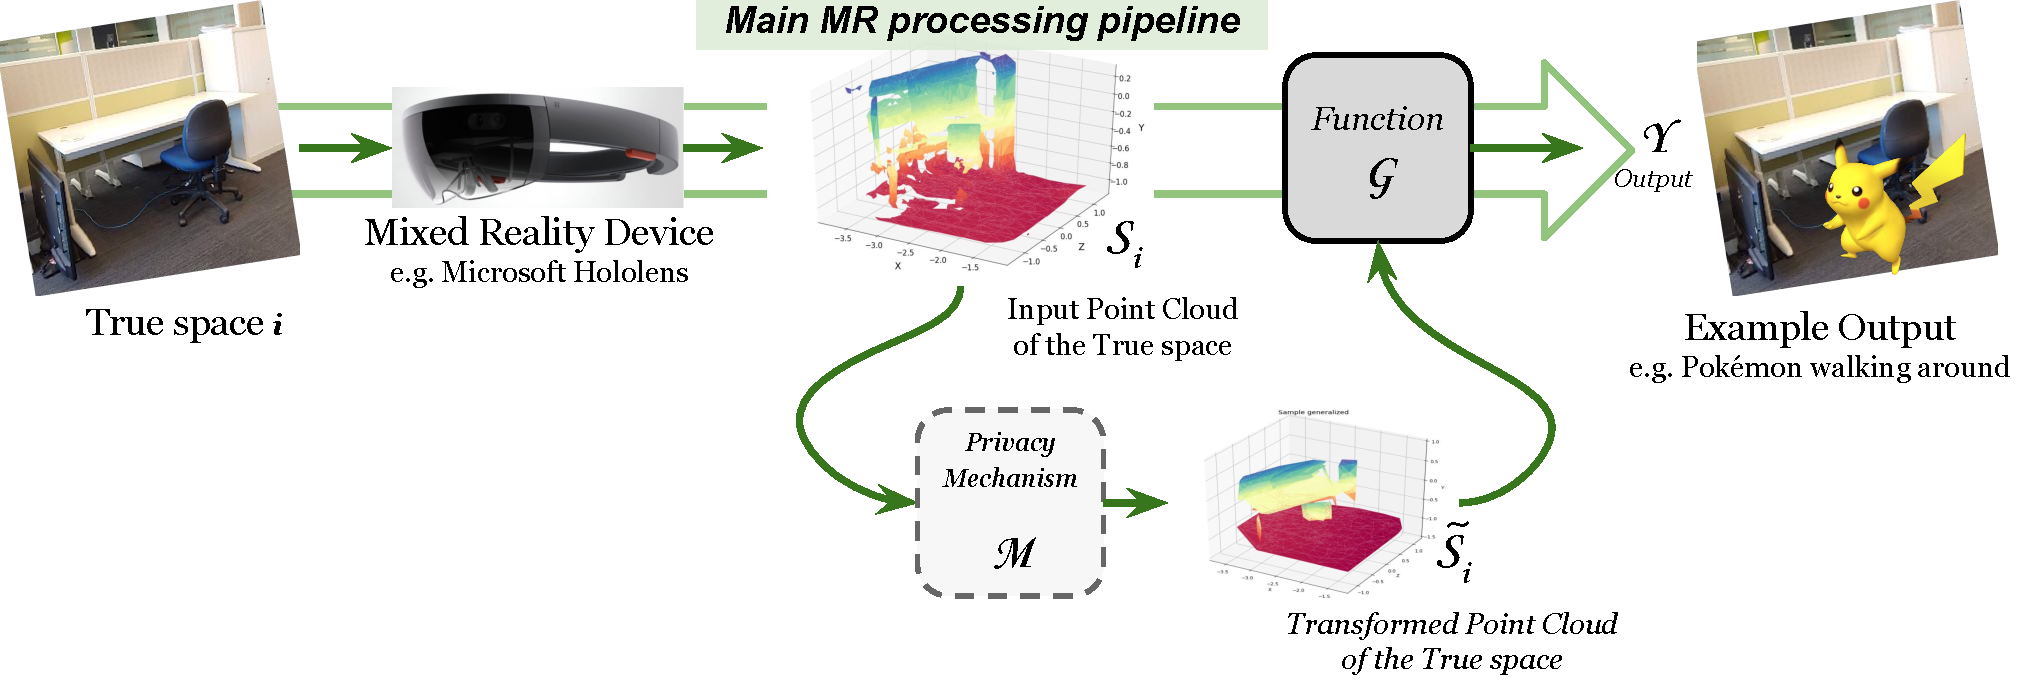
\includegraphics[width=\columnwidth]{figures/adversary-model-pipeline-v6-revised-b.pdf}
		\caption{\small Inserting an intermediate privacy-preserving mechanism $M$ which aims to prevent spatial inference}
		\label{fig:with-privacy-mechanism}
	\end{subfigure}
	\vspace{-3mm}
    \caption{\small AR/MR pipeline diagrams with (a) an attacker, and (b) an introduced intermediary privacy mechanism.}
	\label{fig:adversary-model-pipeline}
	\vspace{-3mm}
\end{figure}

%\textbf{Why 3D?} 
%Furthermore, despite 3D data being a structural representation of the real world, 3D data is perceptually latent from the users. With images and video, what the ``machine sees'' is what the ``user sees'' and a great deal of privacy work have been done on these data forms. Contrariwise, in MR, the experience is exported as visual data (e.g. objects augmented on the user's view) while the underlying spatial mapping, and its extent, as well as the density of the captured points, is not exposed to the users: what the machine sees is different--arguably, even more--than what the user sees. That is, the digital representation of the physical world is not exposed to the user and that the user is oblivious about the captured spatial mapping data. This inherent perceptual difference creates a latency from user perception and, perhaps, affects--or the lack thereof--how users perceive the sensitivity of 3D information.

Aside from the the spatial structural information, the mapping can also include 3D maps of objects within the space. It can also reveal the location of the user: the general location as well as the user's location within the space. Similarly, most users are oblivious about the various information that are included in the spatial maps captured and stored by MR platforms.

\section{Related Work}\label{sec:related-work}

As majority of the work on MR have been focused on delivering the technology, only recently have there been efforts in addressing the security, safety, and privacy risks associated with MR technology. Thus, it is important to start designing and developing \textit{privacy-enhancing technologies} (PETs) especially those that can be applied to the MR use case. Several MR-related PETs that have been proposed in the literature--primarily utilizing \textit{sanitization} and information \textit{abstraction}--are listed in \cite{deguzman2018security}. %To maintain and control the utility of information, 

%\paragraph{Approaches to visual data protection}\label{rrw:vision} Most of the earlier PETs for MR were primarily focused on \textit{visual} information (i.e. image and video) \textit{sanitization} \cite{jana2013scanner,raval2014markit, roesner2014world, aditya2016pic, raval2016you, shu2016cardea, li2016privacycamera, zarepour2016context, steilPrivaceye2018}. Aside from these are \textit{abstraction} approaches to privacy protection. In the specific 3D use case, significant work have been done on protections involving abstracting physiological information \cite{jana2013enabling, figueiredo2016prepose} using the idea of \textit{least privilege} \cite{vilk2014least,vilk2015surroundweb}. A very recent work also utilized the idea of least privilege to apply visual abstractions for mobile MR \cite{deguzman2019safeMR}. However, most of these abstraction approaches are only targeted over specific input types such as physiometric information (i.e. faces, user gestures, and so on), and have not specifically provided protection against spatial recognition attacks. On the other hand, all the sanitization approaches are all focused on post-captured images which can still pose security and privacy risks; moreover, they have only been applied on the wide use case of visual capture devices and not on the specific MR use case.

\paragraph{Approaches to 3D data protection}\label{rrw:3d}
Two works have started to look into and expose the actual risks brought about by unprotected and indefinite access to 3D data by MR applications. Using machine learning, original scenes can be revealed from structure from motion (SfM) 3D point cloud data with additional sparse SIFT or other photometric information \cite{pittaluga2019revealing}. A concurrent work focused on presenting a privacy-preserving method of pose estimation to counter these risks. It removes the necessity for 3D point cloud data by instead using 3D line cloud--effectively obfuscating 3D structural, i.e. geometrical, information--during pose estimation \cite{speciale2019privacy}; however, the 3D line cloud approach only addresses the pose estimation functionality and does not present the viability of its usability for surface or object detection which is necessary for a virtual object to be rendered or ``anchored'' onto. Thus, it would still be necessary for 3D point cloud data to be exposed but, perhaps, with some privacy-preserving transformations to hide sensitive content and further prevent spatial recognition. %Furthermore, even with the absence of additional photometric information, spatial location of 3D point cloud data can still be recognized given that adversaries have access to an ensemble of historical 3D point cloud data \cite{deguzman2019firstlook}. 

\section{3D SPATIAL privacy}

Our earlier work provided preliminary evidence of how easy it is for an adversary to infer the location of spaces from captured 3D data \cite{deguzman2019firstlook}. And how, even with spatial generalization (i.e. the 3D space is generalized in to a set of planes), spatial inference is still possible at a significant success rate, i.e. $P_{success}\geq0.2$ for spaces with radius $r\geq 0.5$meters. We have extended this work with an improved attacker that not only \textit{recognizes} the space, i.e. \textit{inter}-space inference, but also infers the user's location \textit{within} the space, i.e. \textit{intra}-space inference. %To construct the attacker, we build up on existing place recognition methods that have been applied on 3D lidar data and modify it to be usable for the scale on which 3D data is captured by MR platforms. Then, we present spatial generalizations with conservative releasing as a privacy approach. %We also utilize an extended dataset that includes various indoor and outdoor scenes.

\begin{figure}[t]
	\centering
	%\vspace{2mm}
	\begin{subfigure}{0.48\columnwidth}
		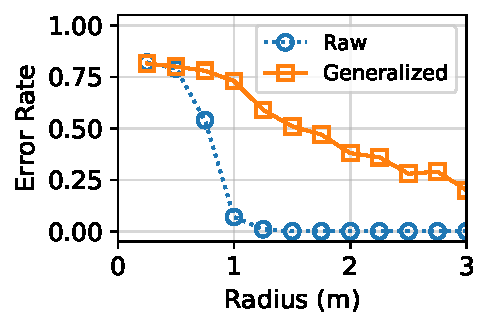
\includegraphics[width=\columnwidth]{figures/cdng-partial-interspace.pdf}
		\vspace{-5mm}
		\caption{\small Inter-space success rate}
		\label{fig:partial-interspace}
    	%\vspace{3mm}
	\end{subfigure}
	\begin{subfigure}{0.48\columnwidth}
		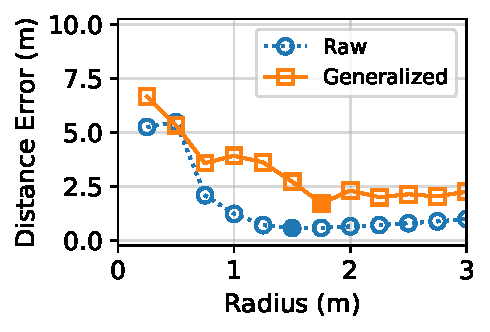
\includegraphics[width=\columnwidth]{figures/cdng-partial-intraspace.pdf}
		\vspace{-5mm}
        \caption{\small Intra-space distance error}
		\label{fig:partial-intraspace}
	\end{subfigure}
	\vspace{-3mm}
    \caption{\small Adversarial inference performance as we vary the size of the revealed space}
	\label{fig:partial-performance}
	\vspace{-3mm}
\end{figure}

\begin{figure}[t]
	\centering
	%\vspace{2mm}
	\begin{subfigure}{0.61\columnwidth}
		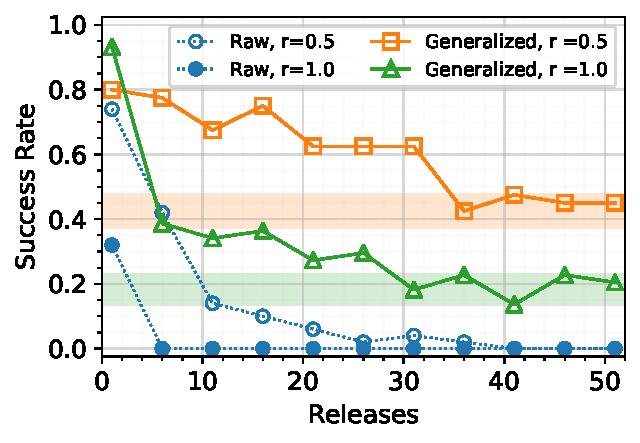
\includegraphics[width=\columnwidth]{figures/cdng-successive-interspace.pdf}
		\vspace{-5mm}
		\caption{\small Inter-space success rate\newline }
		\label{fig:partial-interspace}
    	%\vspace{3mm}
	\end{subfigure}
	\begin{subfigure}{0.37\columnwidth}
		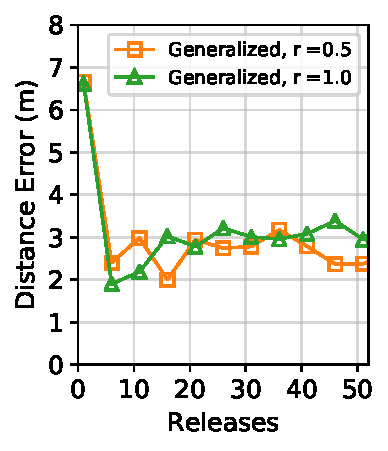
\includegraphics[width=\columnwidth]{figures/cdng-successive-intraspace.pdf}
		\vspace{-5mm}
        \caption{\small Intra-space distance error}
		\label{fig:partial-intraspace}
	\end{subfigure}
	\vspace{-3mm}
    \caption{\small Adversarial inference performance as we \textbf{release} more of the space}
	\label{fig:partial-performance}
	\vspace{-3mm}
\end{figure}

We measure the privacy of the released point cloud in terms of the performance error on these two levels of inference. For inter-space inference, we use the inference error rate directly, while, for intra-space inference, we use the distance error from the true position.

To the best of our knowledge, we are the first to expose spatial privacy risks on 3D spatial data captured by MR platforms. We have demonstrated how easy it is to extend the scope of 3D recognition algorithms to be used as an attacker in the MR scenario. To this end, we summarize the major contributions of this work as follows:

\begin{enumerate}%[leftmargin=*]
	\item First, we formalize the \textit{3D spatial privacy problem} and define the privacy and utility metrics specific to 3D MR data.
	\item We present an \textit{3D adversarial inference model} that reveals the general space of a user, i.e. inter-space inference, and their specific location within the space, i.e. intra-space inference or, commonly, tracking attack.%, e.g. point sampling factor by 3.
	%In particular, we define the 3D adversarial inference using the well-established Bayesian inference as basis.
	\item Using 3D point cloud data collected from Microsoft HoloLens, which is also the same 3D data representation format for Google's ARCore and Apple's ARKit, we demonstrate that 3D spatial inference attacks are possible on these MR platforms.
	\item We demonstrate that the insufficient protection provided by spatial generalizations can be improved by conservatively releasing the generalizations; specifically, we control the release of plane generalizations rather than giving out the generalizations entirely. %However, %as well as the 	negative impact on utility of these generalizations. 
	\item We also show that we can get better data utility with a smaller size of space while providing adequate privacy. 
	\item Lastly, we present an in depth analysis over a realistic scenario when user spaces are successively released and experimentally determine the minimum number of releases, and planes that prevents spatial inference, both inter-space and intra-space.
	%\item Lastly, we 
	%delaying release of small partial spaces (with radius $r<0.25$) and maintaining a low number of planes, i.e. $< 5$, can delay inference and potentially provide privacy. %in conjunction with a localized generalization.
	%higher number of planes can be inferred more precisely but does not necessarily improve recall or reduce error rate.
	%\item Lastly, we show the \textit{memory compactness} of 3D data which emphasizes how adversaries can create lightweight 3D inference models of user spaces.
\end{enumerate}

%RETURN HERE AFTER REARRANGING ALL THE SECTIONS.

The rest of the paper is organized follows. First, we discuss the related work in \S\ref{sec:related-work}. Then, \S\ref{sec:framework} presents the theoretical framework of spatial privacy problem and the definitions of the elements of the framework as well as the adversary model. In \S\ref{sec:privacy-preservation}, we describe the various information reduction techniques we can employ to prevent spatial inference. Likewise, we describe in \S\ref{sec:3d-space} the different description and inference methods an adversary may utilize for spatial inference. We present the evaluation methodology in \S\ref{sec:methodology} to investigate the viability of privacy methods we employ over varying experimental setups. The results are presented in \S\ref{sec:results} followed by the discussion in \S\ref{sec:discussion}. We conclude the paper in \S\ref{sec:conclusion}. % and \S\ref{sec:future_work}, respectively. 

\section{Conclusion}\label{sec:conclusion}
Currently, MR services are provided full and indefinite access to the 3D spatial information, i.e. 3D point cloud data, captured by an MR-capable device. In this work, we highlight that the risks associated to the indefinite access of applications to these 3D point cloud data. Our preliminary work have presented preliminary evidence of these risks \cite{deguzman2019firstlook}. We have earlier demonstrated how a descriptor-based inferrer can be used for 3D spatial inference. Using this inferrer, we can identify, i.e. inter-space inference, the current space of the MR user using the 3D point cloud information provided by the MR device to the MR service. We enhance this inter-space inferrer in this work.

Furthermore, we have extended the capability of the inferrer to also reveal the exact location within the space, i.e. instra-space inference, of the user. Our validation results reveal that, unsurprisingly, raw 3D point cloud data readily reveals the specific location of spaces with average intra-space error of as low as $1 m$. And that naive spatial generalizations, i.e. using the RANSAC plane-fitting algorithm, is still inadequate.%cannot protect against this kind of inference.

Therefore, it is necessary to provide users with a form of protection, i.e. privacy preserving 3D point cloud releasing. %This was the primary goal of this work.
This time, we have demonstrated that we can enhance the protection from plane generalizations by simply conservatively releasing the generalized planes provided to applications. Our emulated experimental investigation reveals that we can reveal upto 13 planes and avoid inter-space inference half the time. Specifically, with such very conservative releases, the success rate of an (inter-space) inferrer is no better than a random guess. And, for the occasions that the adversary correctly recognizes the space, the intra-space location can be off by at least 3 meters. Moreover, we have shown a quantification of how much we can improve both $\Pi_1$ and $\Pi_2$ by reducing the size of the partial spaces to be revealed. Consequently, in terms of data utility $Q$, a smaller size is anyway preferred to provide good (i.e. low) $Q$. %Similarly, for intra-space inference, for those correctly ``guessed'' spaces will be off by 5 meters or farther.

Overall, these results provides quantities, i.e. thresholds, that allows us to potentially protect users and their spaces as they user MR services. Moreover, we have only utilized simple approaches to spatial privacy protection. Generalization are already implemented in most MR platforms. Thus, what remains is the implementation of conservative plane releasing to provide protection.
%For future work, a practical investigation can provide us with the impact of our presented simple approach on usability of the MR application provided with such generalizations. Furthermore, we also plan to investigate the effectiveness and impact of adding plane perturbations, i.e. translation and/or rotation. %Future work, 1) perturbations, i.e. plane translation and/or rotation; 2) practically demonstrate a proof-of-concept using at least an HMD and a mobile device, then, measure QoE. A practical investigation can provide us with actual user feedback on whether our approach affects the usability of the application or not.


\bibliographystyle{ACM-Reference-Format}
\bibliography{bib_all.bib}

\end{document}



